%!TEX root = Thesis.tex

\chapter{Experimental Results}
\label{cha:experimental_results}

We make extensive use of three components: visual car detection,
parking lot modeling and planning.

\section{Visual Car Detection}
\label{sec:visual_car_detection}

We start this section by describing the dataset that we utilize to train the
car detector. A training dataset plays a crucial part in any detection
algorithm. In order to train the visual car detector we assemble a training
dataset that consists of a number of positive (containing cars) and negative
(images not containing cars) examples.

For the reason that the car's view depends on the angle of view, we assemble
positive training data for different angles of the cars. We prepare training
samples for four different views of the cars --- front, back and both left and
right sides.

The sides of the car are invariant under the mirror transformation. Front and
back of the car, though different to human point of view, seem to be similar
in the HOG visualization. Therefore, the corresponding datasets can be
combined into one.

\begin{figure}[b]%
\centering
\subfloat{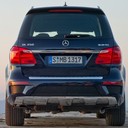
\includegraphics[width=0.14\textwidth]{pictures/pos_1.png}}
\hspace{2mm}
\subfloat{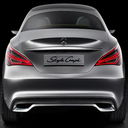
\includegraphics[width=0.14\textwidth]{pictures/pos_2.png}}
\hspace{2mm}
\subfloat{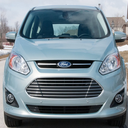
\includegraphics[width=0.14\textwidth]{pictures/pos_3.png}}
\hspace{2mm}
\subfloat{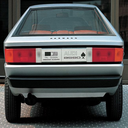
\includegraphics[width=0.14\textwidth]{pictures/pos_4.png}}
\hspace{2mm}
\subfloat{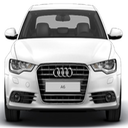
\includegraphics[width=0.14\textwidth]{pictures/pos_5.png}}
\hspace{2mm}
\subfloat{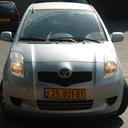
\includegraphics[width=0.14\textwidth]{pictures/pos_6.png}}\\
\subfloat{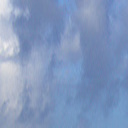
\includegraphics[width=0.14\textwidth]{pictures/neg_1.jpg}}
\hspace{2mm}
\subfloat{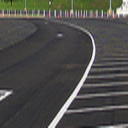
\includegraphics[width=0.14\textwidth]{pictures/neg_2.jpg}}
\hspace{2mm}
\subfloat{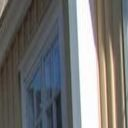
\includegraphics[width=0.14\textwidth]{pictures/neg_3.jpg}}
\hspace{2mm}
\subfloat{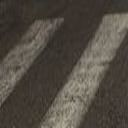
\includegraphics[width=0.14\textwidth]{pictures/neg_4.jpg}}
\hspace{2mm}
\subfloat{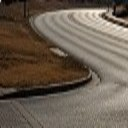
\includegraphics[width=0.14\textwidth]{pictures/neg_5.jpg}}
\hspace{2mm}
\subfloat{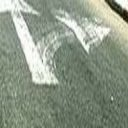
\includegraphics[width=0.14\textwidth]{pictures/neg_6.jpg}}
\caption{Examples of positive and negative training examples for front/rear car detector.}
\label{fig:pos_neg_examples}
\end{figure}

These datasets contain respectively images of sizes $128 \times 128$ pixels
for front/rear car view and $128 \times 64$ pixels for side view. We utilize
682 positive images that contain cars for training the front/rear detector. In
addition to these positive examples we also convene 7972 negative images. The
examples of the positive and negative training datasets are presented in
Figure~\ref{fig:pos_neg_examples}.

The positive examples contain exclusively views of the cars. Each positive
example shows one and only one car. The car occupies the full area of the
image. The photos of the cars depict them centered and seen from the same
angle of view. This is crucial for training a meaningful classifier.

The positive dataset is assembled from different sources: INRIA Car Dataset
by~\citet{inriadata}, Motorway Car Dataset by~\citet{TMEMotorwayDataset} and
various car images found in a public domain via Google.

In order to create the negative set we randomly sample different sized patches
of the given aspect-ratio ($128 \times 128$ and $128 \times 64$ respectively)
from the images that contain no cars. Following the work of~\citet{dalal2005}
we cut false detections that appear in the first runs of training the
classifier with a clipping tool~\cite{imageclipper} and add them to the
negative training dataset.

We use the trained classifier on the images from the camera mounted on the car
or, possibly, any other moving platform. During our experiments we use a
Bumblebee stereo-camera (Figure~\ref{subfig:bumblebee}) pointed to the side of
the Europa robot Obelix (Figure~\ref{subfig:obelix}).

\begin{figure}[t]%
\centering
\subfloat{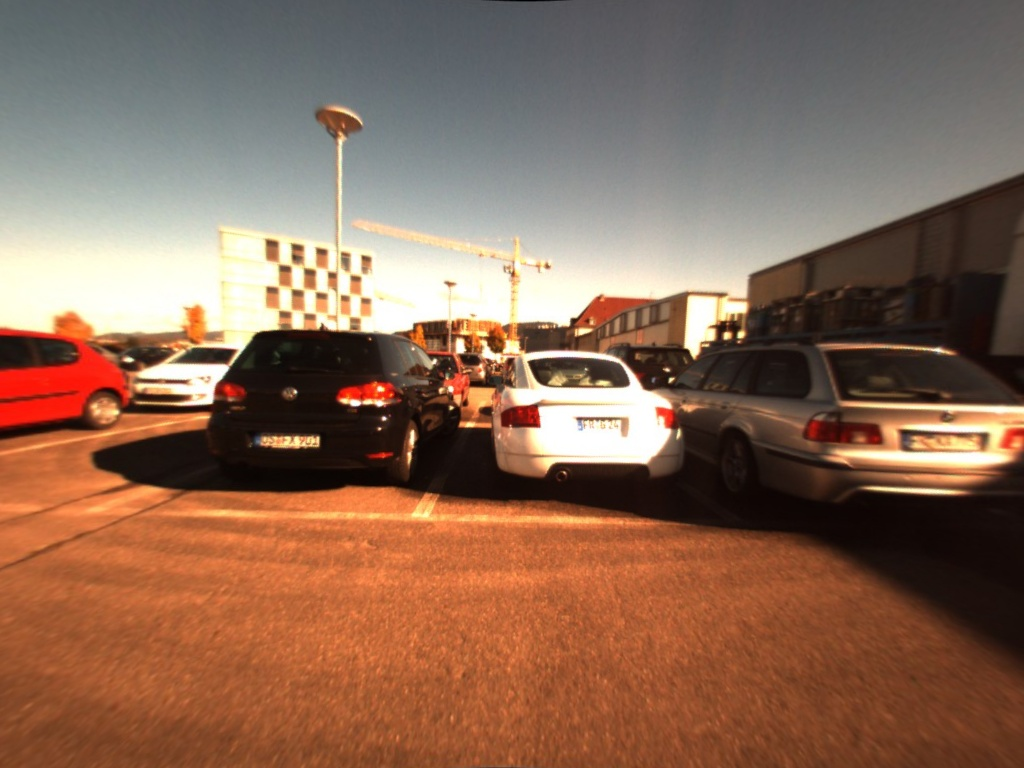
\includegraphics[width=0.31\textwidth]{pictures/left.jpg}}\hspace{2mm}
\subfloat{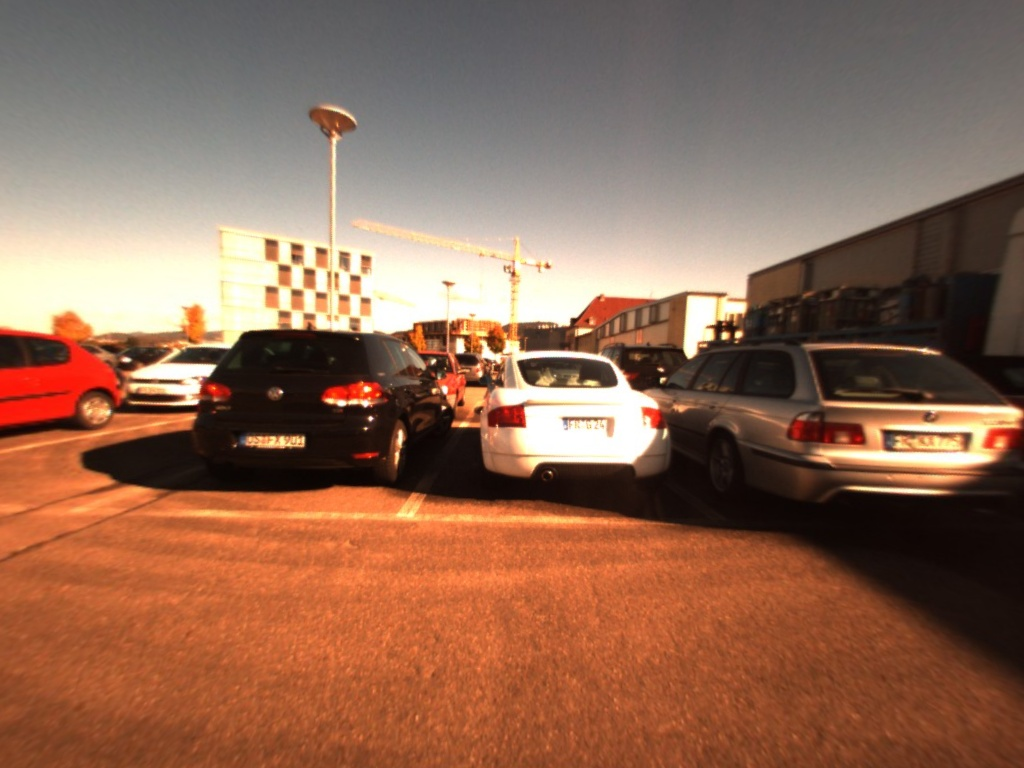
\includegraphics[width=0.31\textwidth]{pictures/right.jpg}}\hspace{2mm}
\subfloat{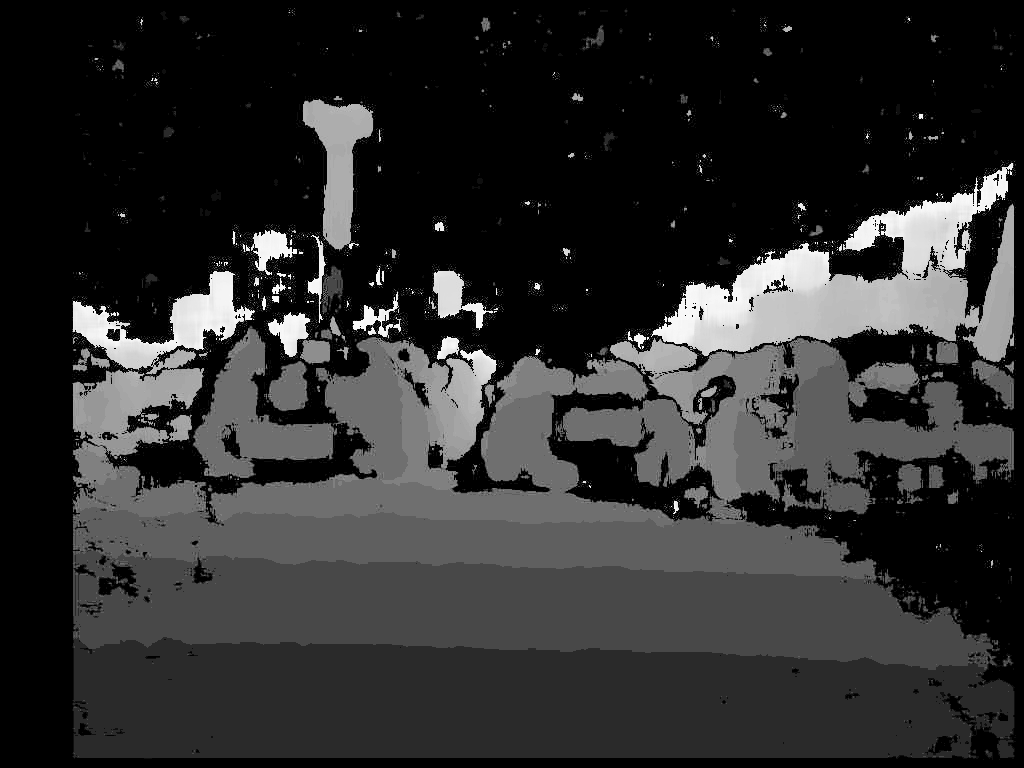
\includegraphics[width=0.31\textwidth]{pictures/depth.png}}\\
\caption{Depth acquired from disparity between stereo images.}
\label{fig:depth_from_disparity}
\end{figure}

We are interested in detections accumulated over time. The same car is seen
from different angles, throughout different (usually consequent) images. We
consider the car to be detected if it has been detected at least once in the
sequence of images, featuring this particular car. With this in mind, the
detection rate for our realization of the approach is approximately 95\%.

The examples of detected cars can be seen in
Figure~\ref{fig:detection_examples}.

\begin{figure}[th]
\centering
\begin{tabular}{cc}
\subfloat[]{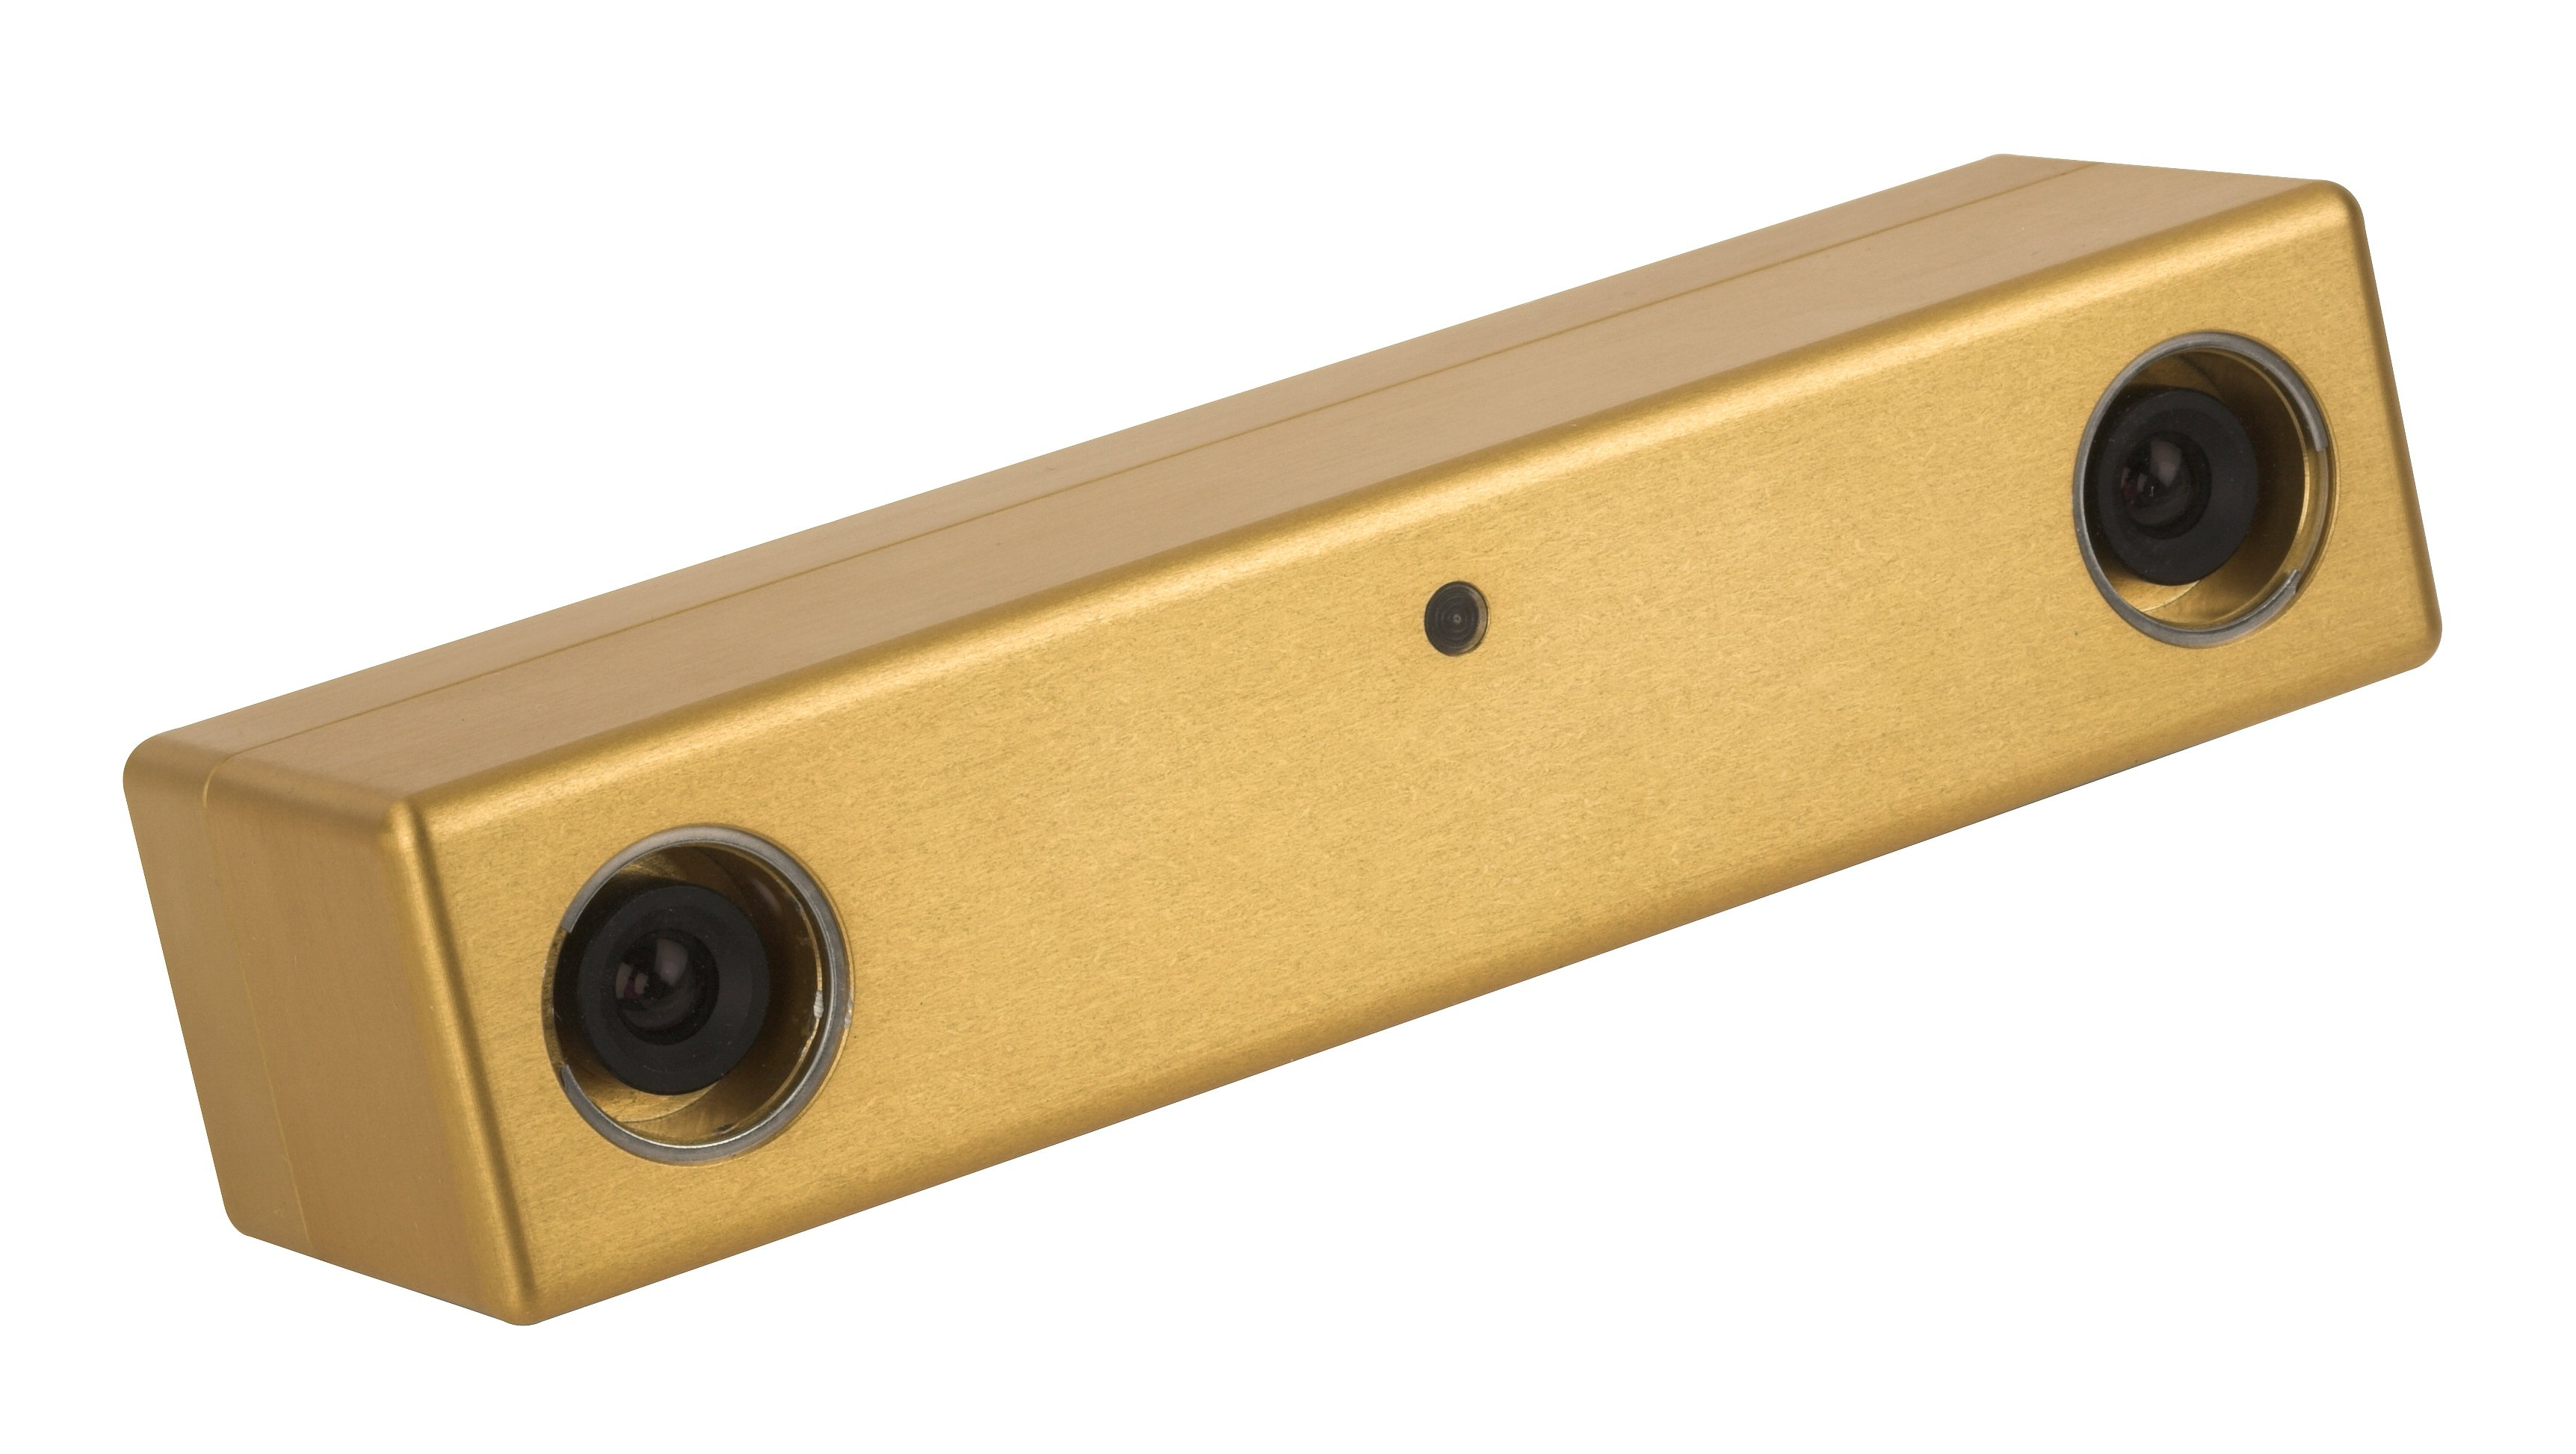
\includegraphics[width=2.5cm]{pictures/bumblebee.jpg}\label{subfig:bumblebee}}\vspace{4mm} \\
\subfloat[]{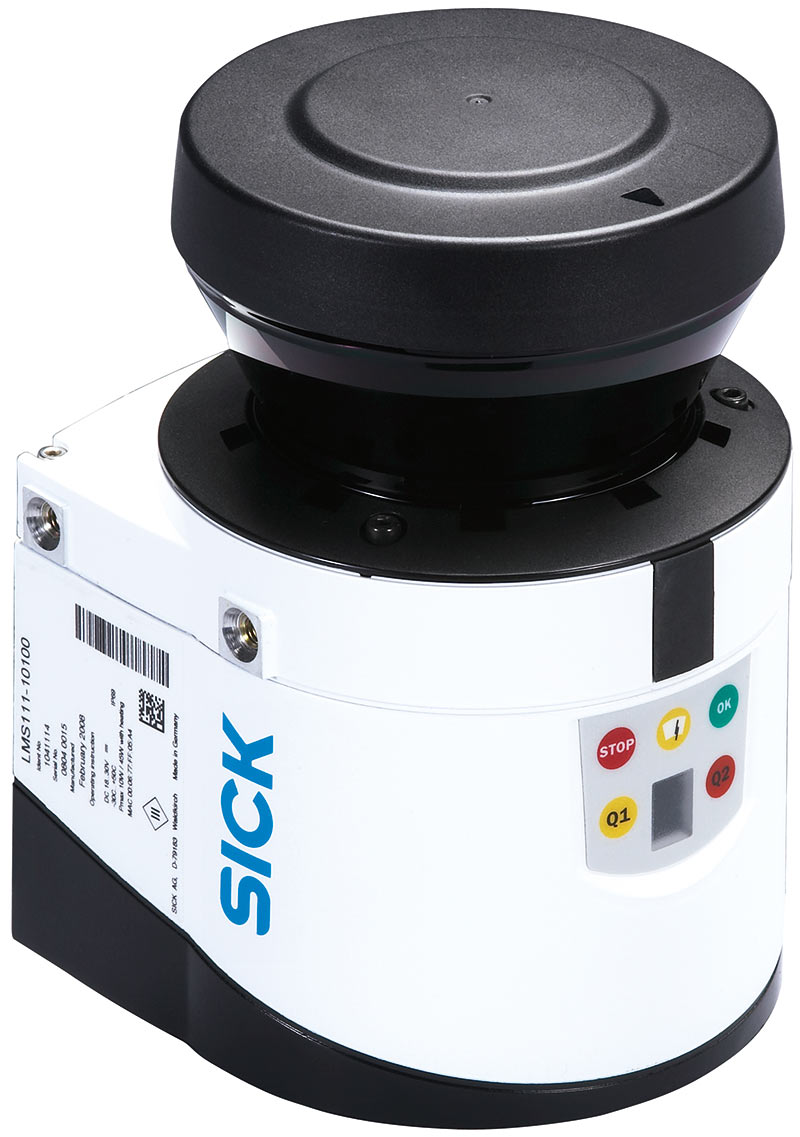
\includegraphics[width=2cm]{pictures/lms_2_0.jpg}\label{subfig:laser}} &
\multirow{-12}[2.5]{*}{\subfloat[]{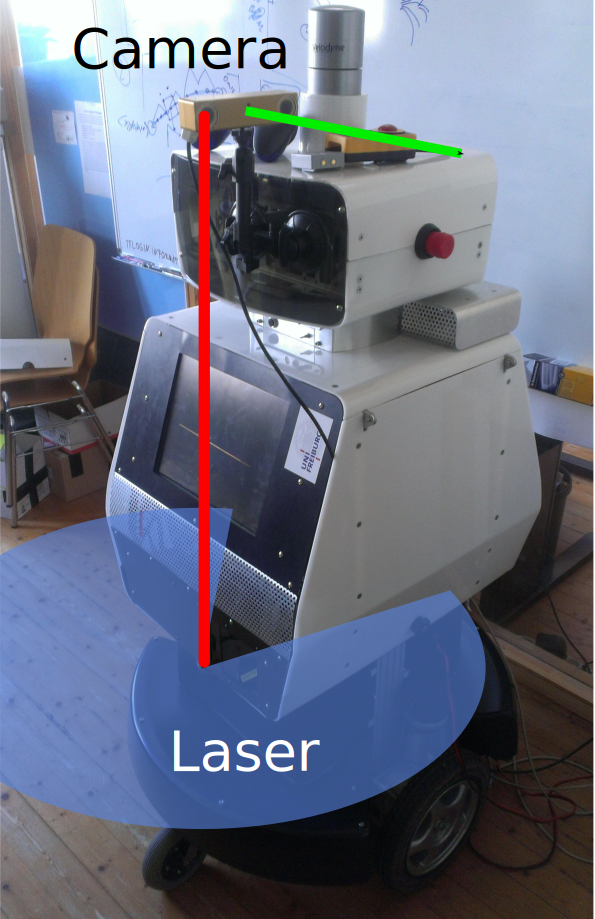
\includegraphics[width=4cm]{pictures/obelix.pdf}\label{subfig:obelix}}} \\
\end{tabular}
\caption{A Bumblebee stereo camera \subref{subfig:bumblebee} and a laser range finder \subref{subfig:laser} mounted on the Obelix robot on the same vertical axis \subref{subfig:obelix}.}
\end{figure}

% section visual_car_detection (end)

\section{Parking Lot Modeling}
\label{sec:parking_lots_modeling}

\begin{figure}[p]%
\centering
\subfloat{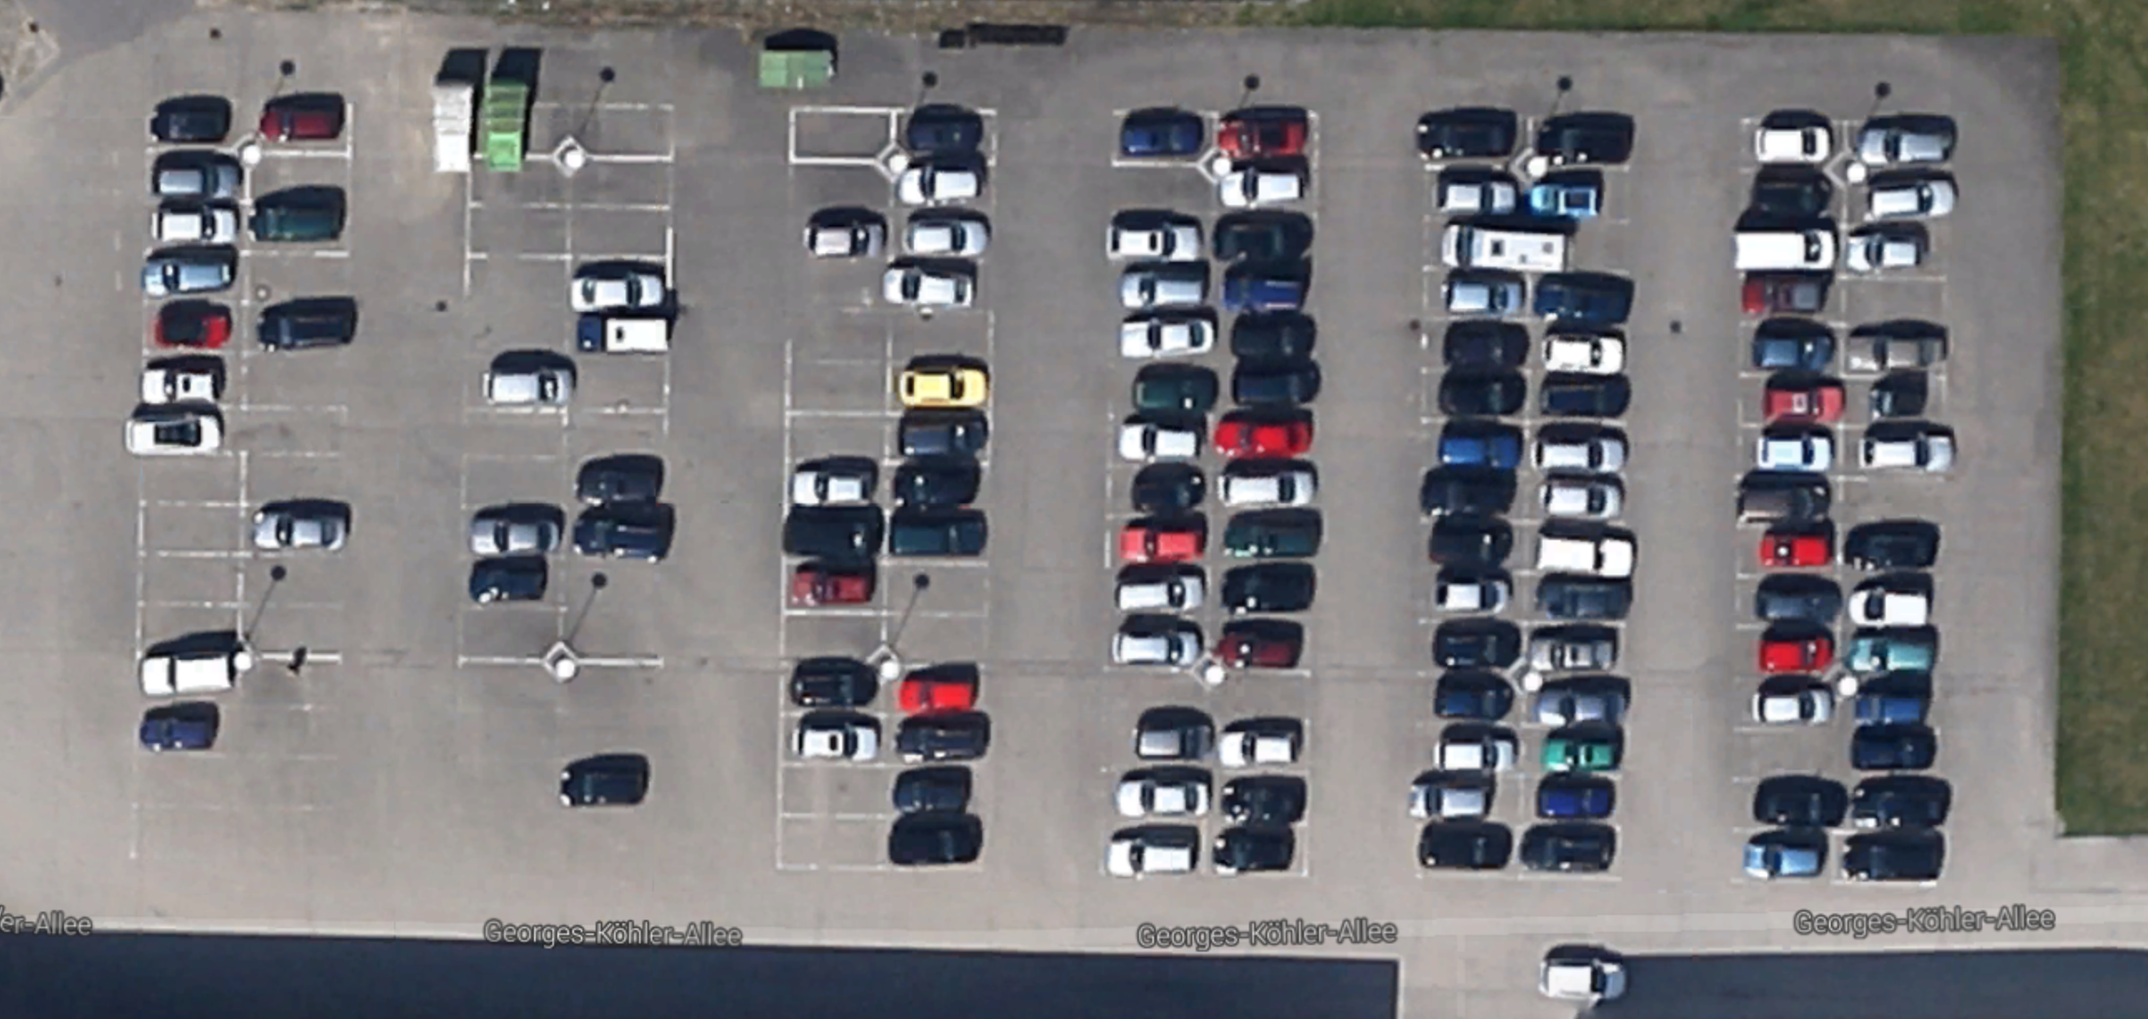
\includegraphics[width=0.7\textwidth]{pictures/google_map.pdf}} \\
\subfloat{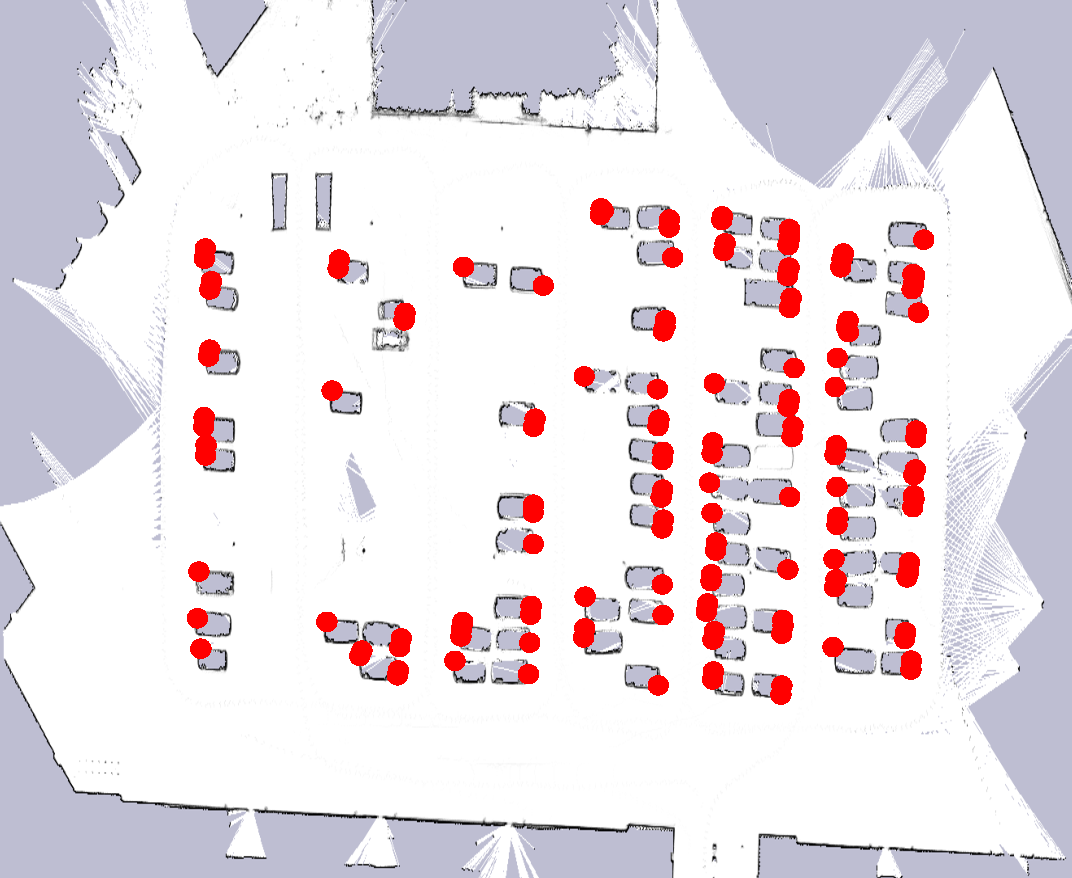
\includegraphics[width=0.7\textwidth]{pictures/laser_fusion.pdf}} \\
\subfloat{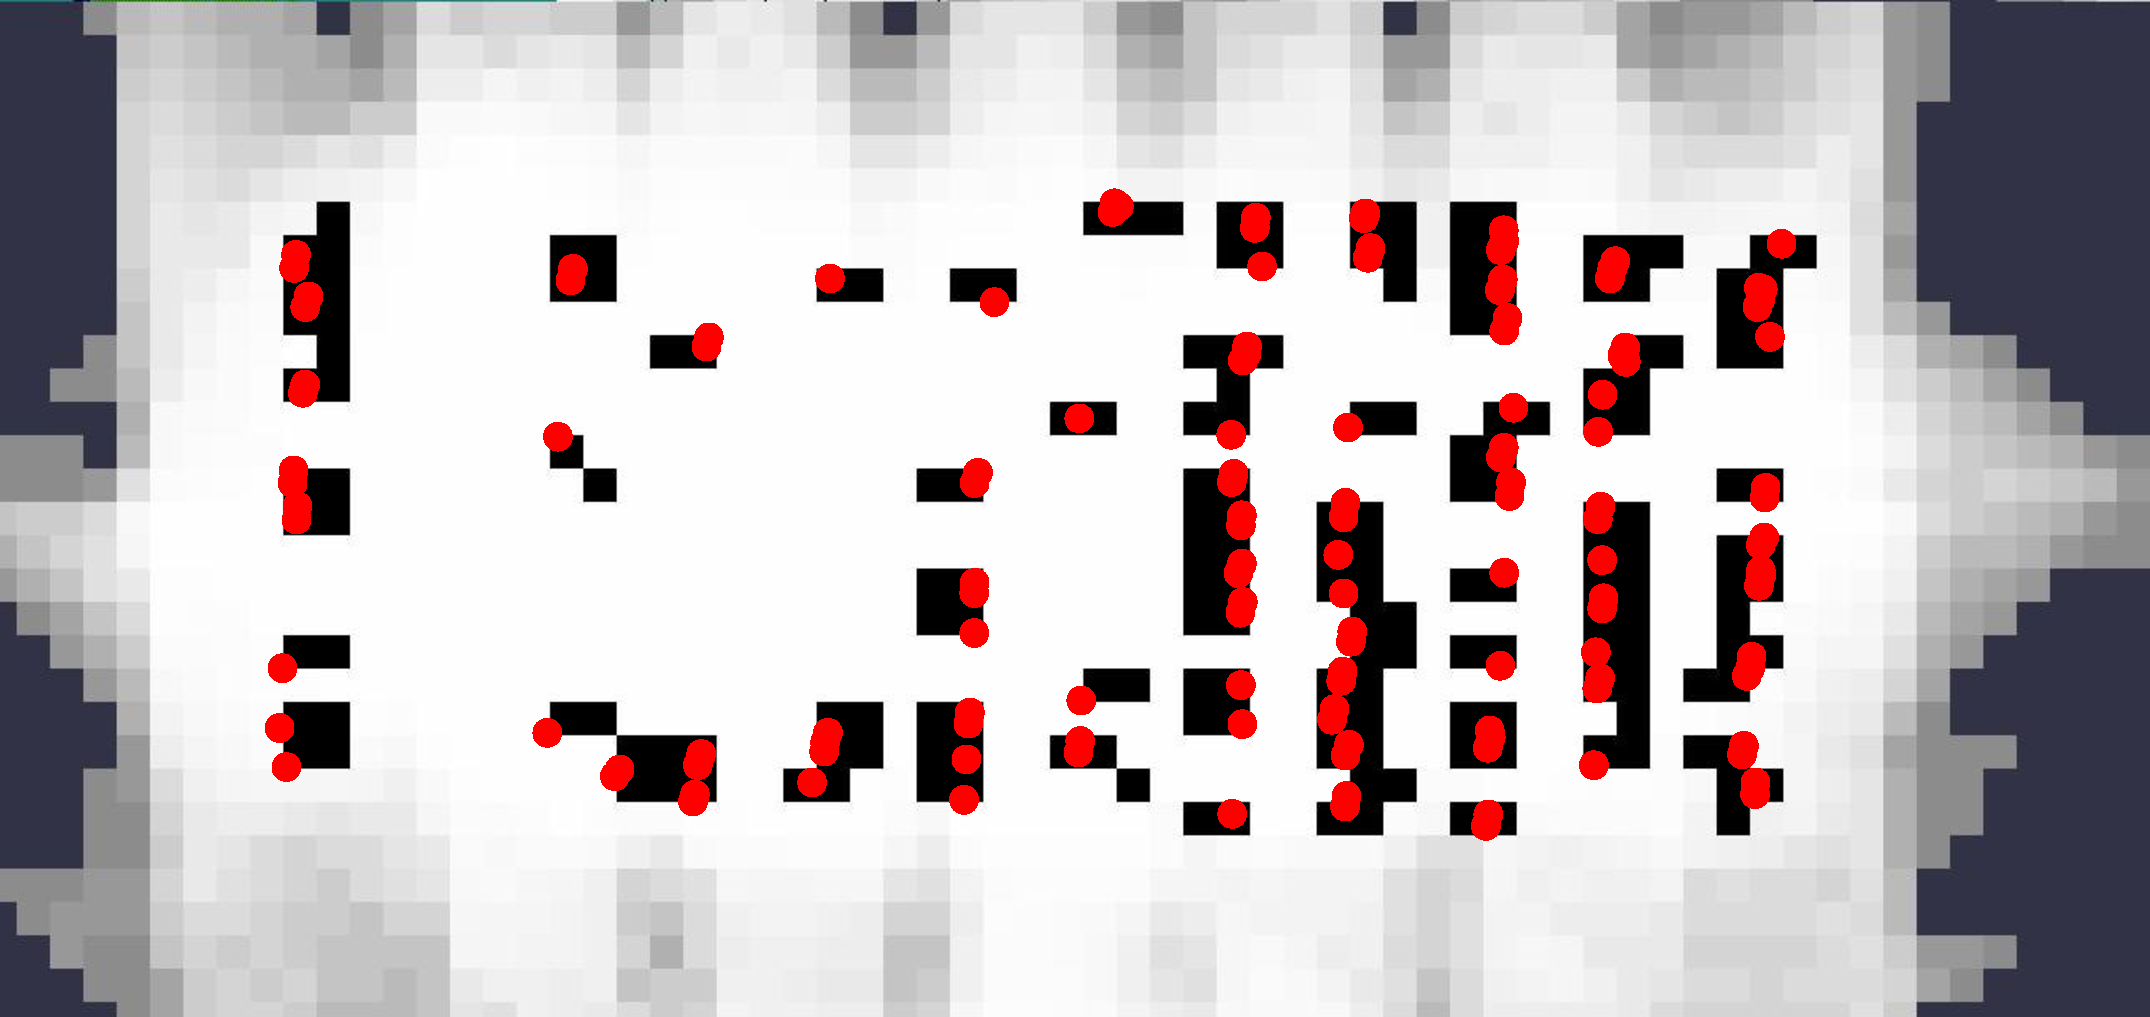
\includegraphics[width=0.7\textwidth]{pictures/occupancy_cars.pdf}} \\
\subfloat{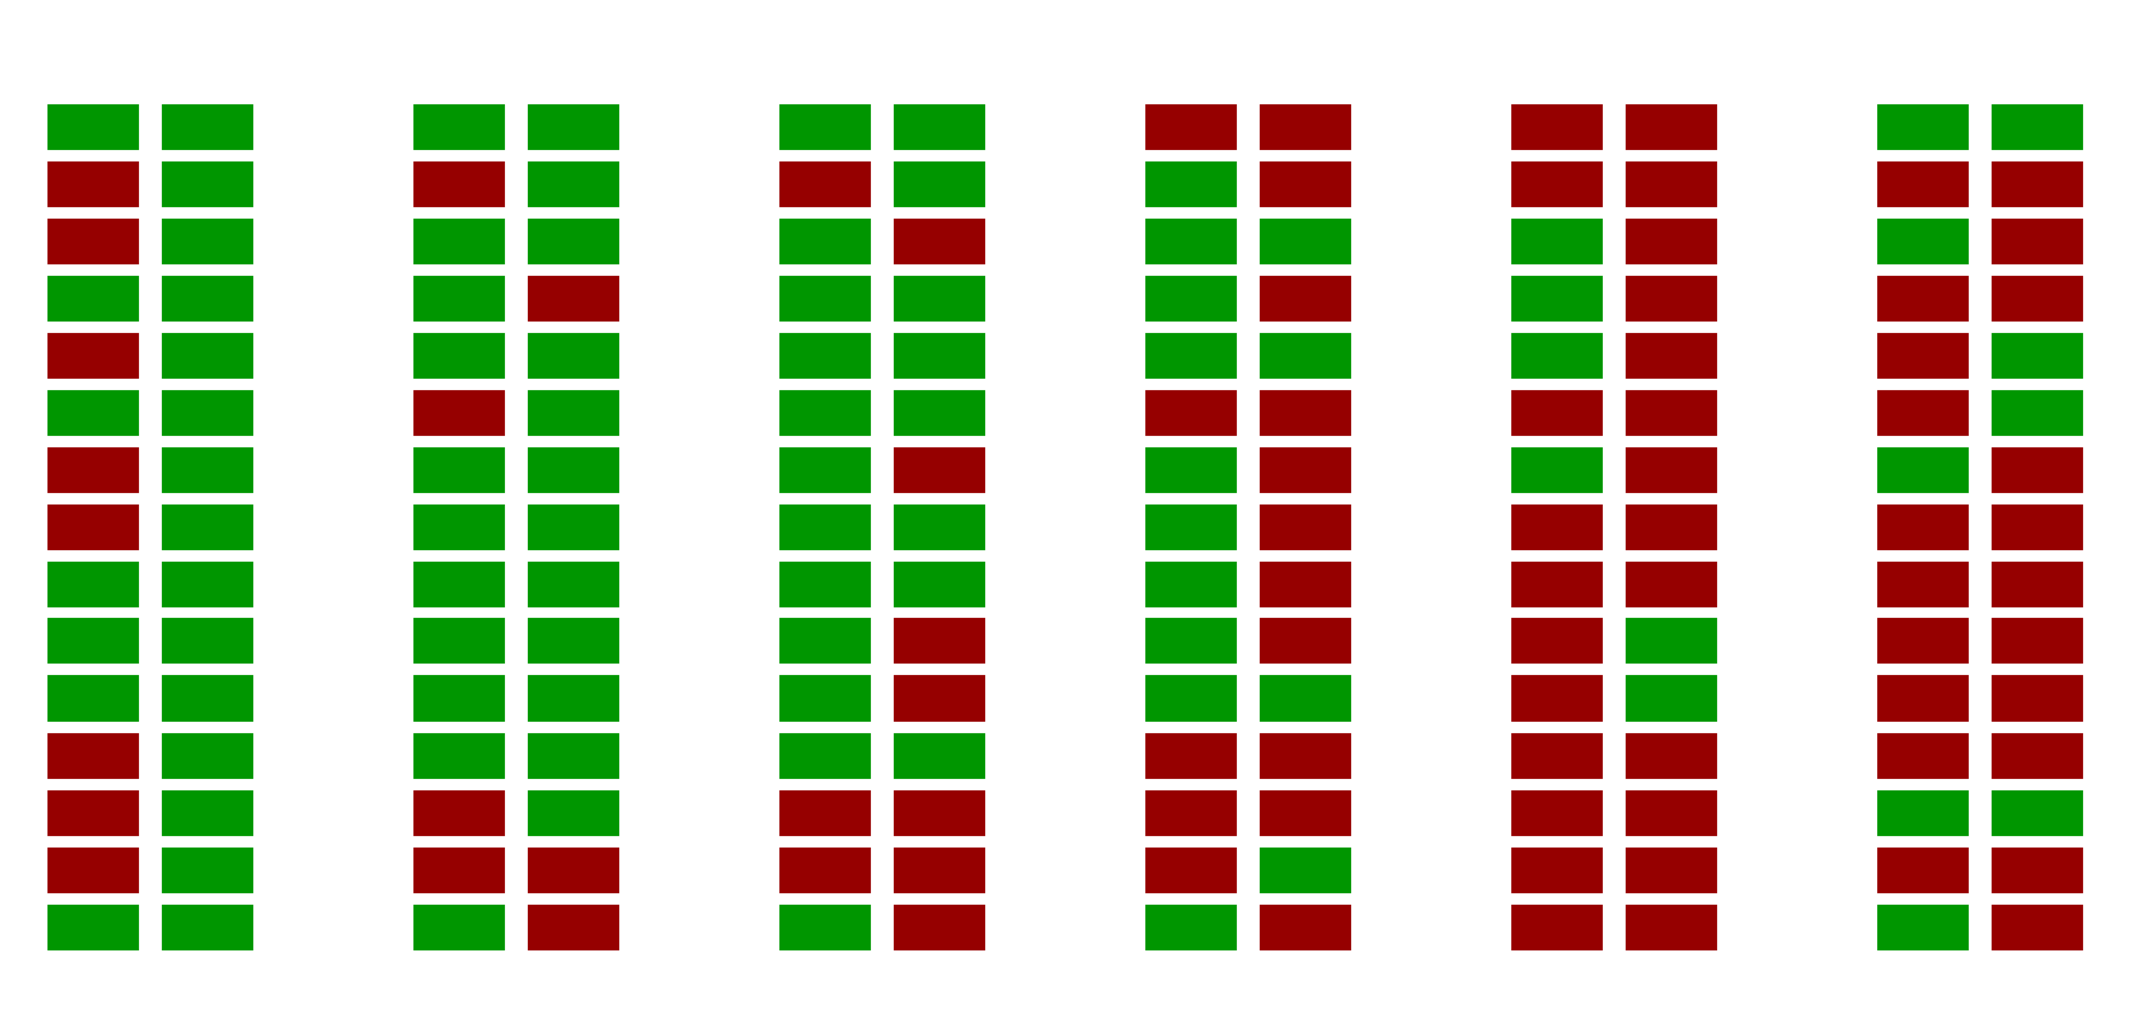
\includegraphics[width=0.7\textwidth]{pictures/parking_lots_detections.pdf}}
\caption{Illustration of different mapping approaches.}
\label{fig:different_mappings}
\end{figure}

We present occupancy data aggregated to the occupancy grids as well as into
the pre-defined parking lot positions. The illustration of differences in the
maps representations can be seen in Figure~\ref{fig:different_mappings}.

The occupancy data is based on the 2D data obtained either from the stereo
cameras (Figure~\ref{fig:depth_from_disparity}) or from laser range finder,
mounted on the robot (Figure~\ref{subfig:laser}). As can be seen in the
figure, the stereo camera is mounted on the same z-axis as the laser range
finder. We search for the endpoints that represent the cars as described in
the section \nameref{sec:perception} of chapter \nameref{cha:our_approach}.

Figure~\ref{fig:depth_from_disparity} shows that the depth information
computed from the disparity information between two stereo images lacks
precision and overall is noisy. Not only this noise is caused by the method of
depth estimation and errors in point association, but it also suffers from the
windows present in almost any car. The windows are transparent which results
in wrong depth measurements falling into the detected region of interest.

As the result of this, we use the laser range finder based depth measurements.
Laser is precise in measuring the distance. Because of its mounting position
on the human knee level, it also does not suffer from the partial transparency
of the cars because the lasers never encounter the cars' windows.

Figure~\ref{fig:different_mappings} shows car detections as red dots. We
produce these detections fusing the laser range finder measurements with the
visual detections as described in Chapter~\ref{cha:our_approach}.

The precision of car position modeling can be seen in
Figure~\ref{fig:different_mappings}. The occupancy grid maps suffer from
discretization errors. We have observed situations when the detections of the
same car fall into different grid cells, causing erroneous map representation.

Another problem with occupancy grid approach is the ad-hoc modeling of the car
orientation. We argue, that using the observation model, as seen in
Figure~\ref{fig:maptest}, yields the orientation of the detected car to be
influenced by the angle from which it is observed. This is the second source
of the errors in the map representation via occupancy grid maps.

% section parking_lots_modeling (end)


\section{Planning}
\label{sec:planning_results}

As can be seen in the previous section, the question of how to use the
occupancy grids in order to build a planner on top of the occupancy
information in them is still open. We thus currently focus on a planner based
upon the pre-defined parking lots positions. However, the planner itself is
generic, which allows to use it in any situation alike. For now we can
manipulate the constant time for taking the next action. It can be seen, that
if this value is set to a very big value, the optimal action for each state is
to park right there just to keep the overall reward positive. If we on the
contrary set this constant to 0, the optimal decision will be to move around
the parking lot until we have found the best (closest to the goal) parking lot
and then try to park there.

The most optimal result is achieved if the cost of moving between the parking
lots by car is the distance between them, divided by the speed of the car.
This makes the algorithms consider a trade-off between shorter routes while
searching for a place and better parking lots, situated closer to the goal,
weighted by the occupancy probability. The next example shows the behavior of
the agent under different current occupancy.

% section planning_results (end)
% chapter experimental_results (end)

\begin{figure}[p]%
\centering
\subfloat{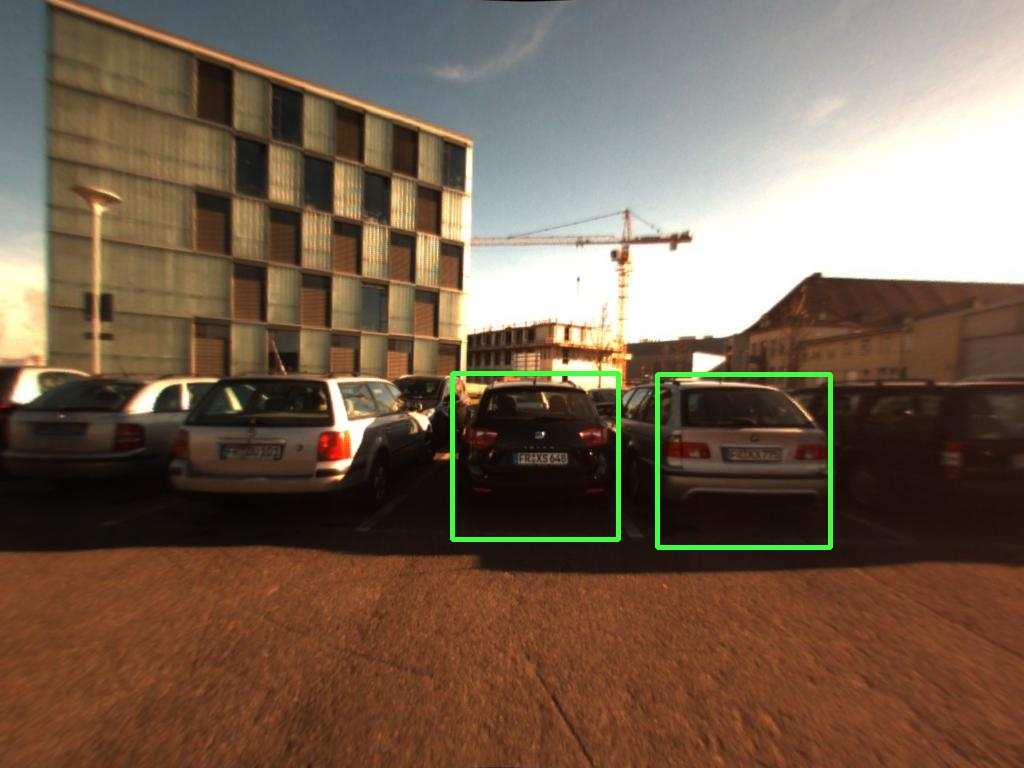
\includegraphics[width=0.31\textwidth]{pictures/det_1.jpg}}\hspace{2mm}
\subfloat{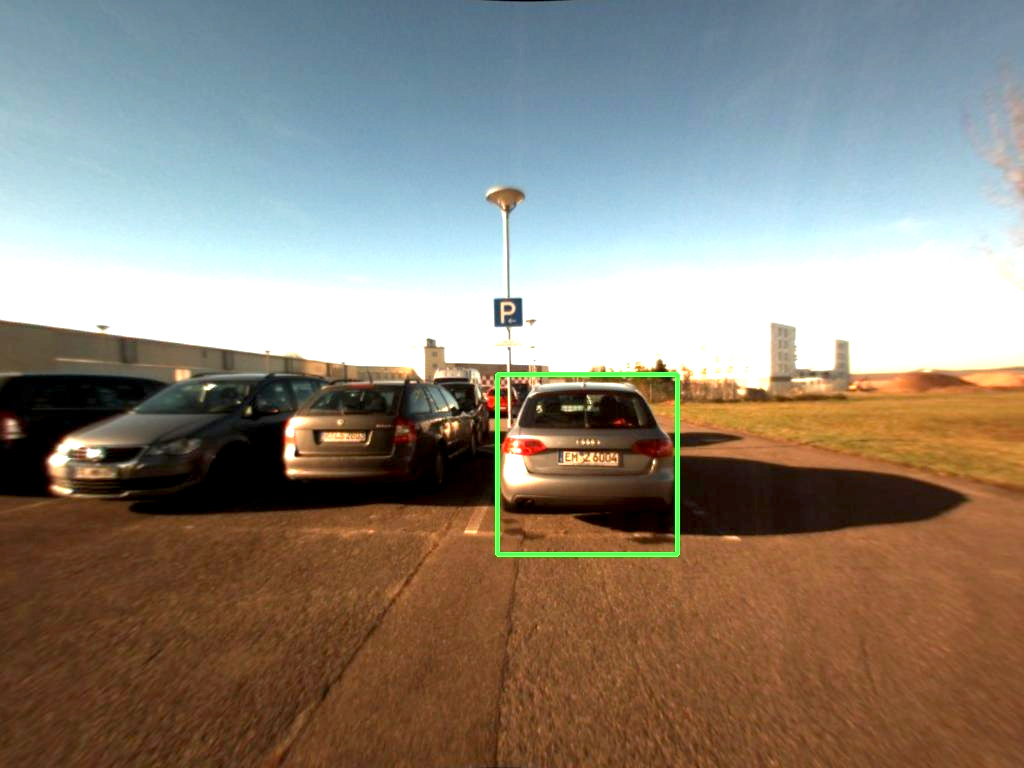
\includegraphics[width=0.31\textwidth]{pictures/det_2.jpg}}\hspace{2mm}
\subfloat{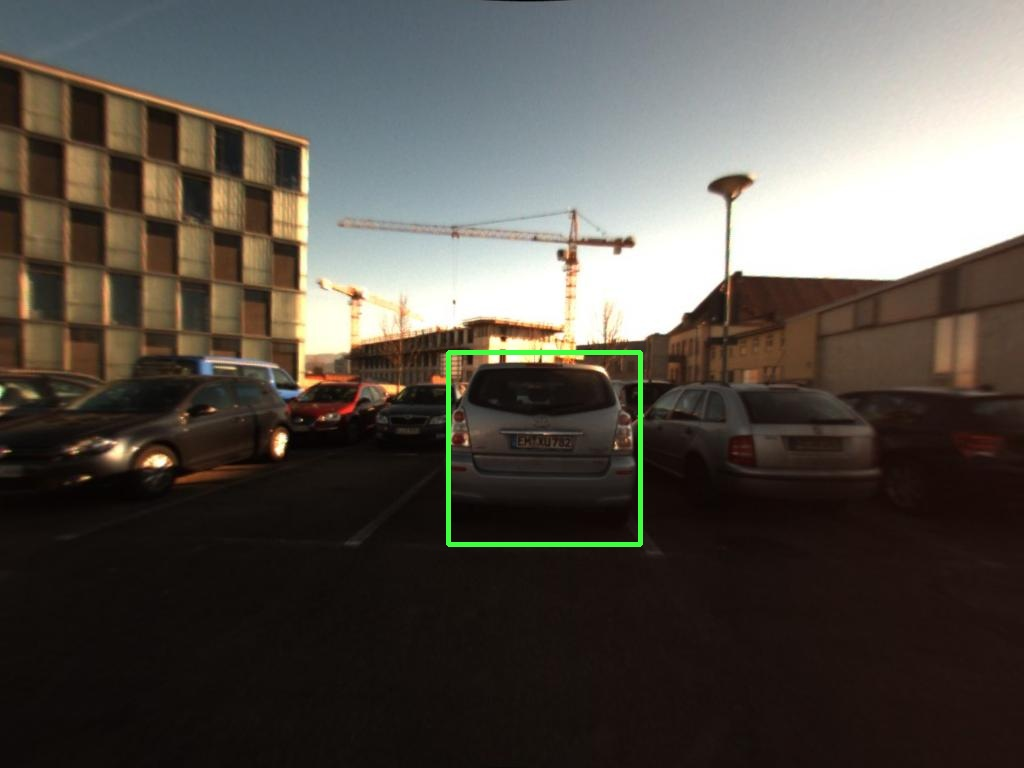
\includegraphics[width=0.31\textwidth]{pictures/det_3.jpg}}\\
\subfloat{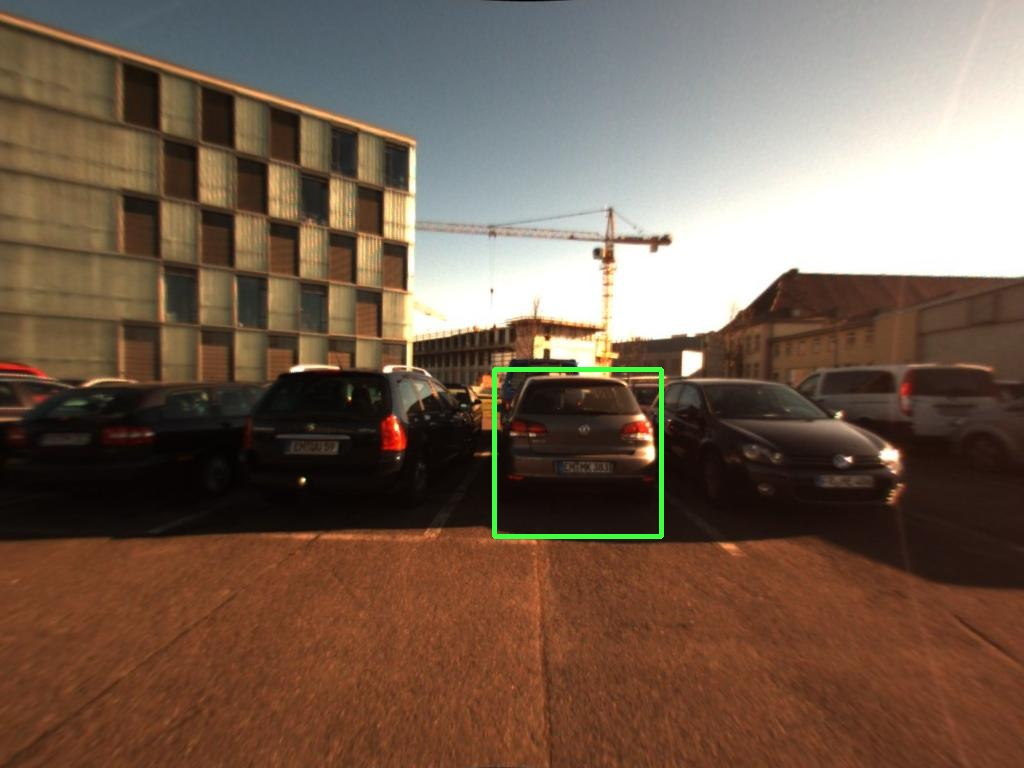
\includegraphics[width=0.31\textwidth]{pictures/det_4.jpg}}\hspace{2mm}
\subfloat{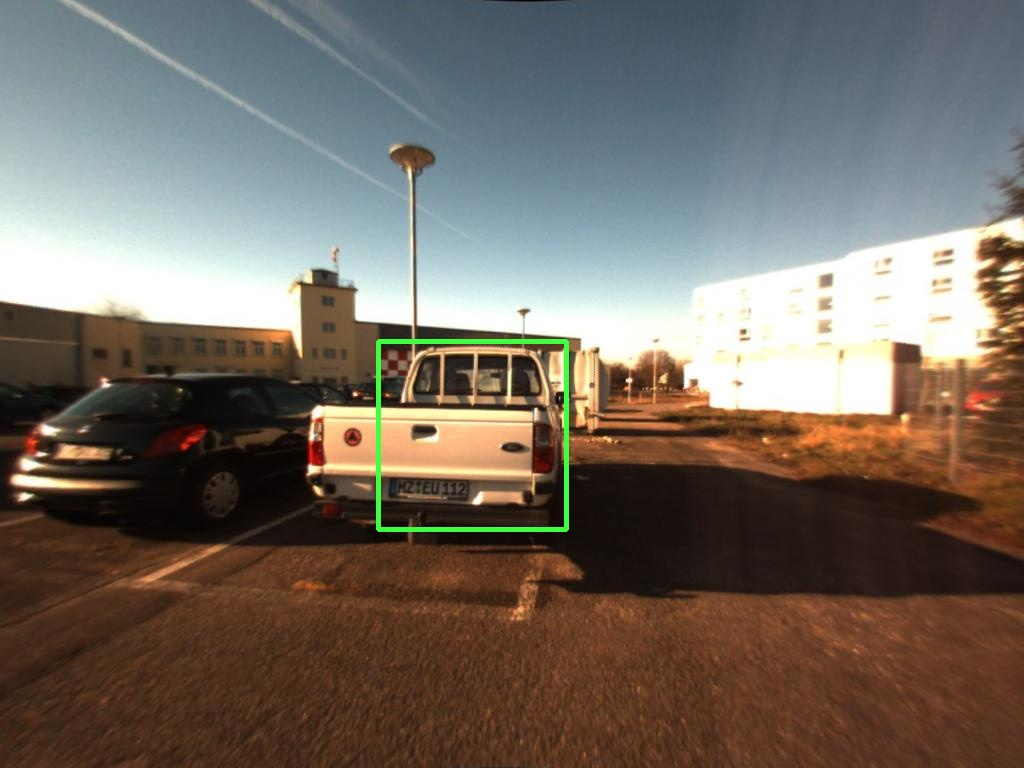
\includegraphics[width=0.31\textwidth]{pictures/det_5.jpg}}\hspace{2mm}
\subfloat{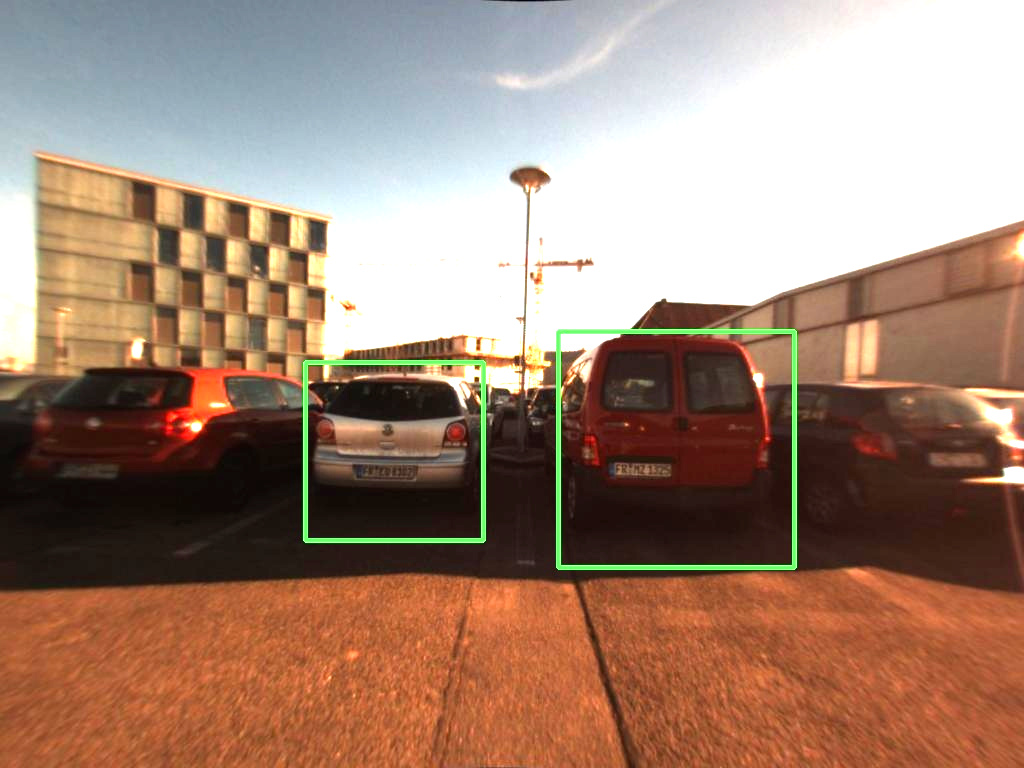
\includegraphics[width=0.31\textwidth]{pictures/det_6.jpg}}\\
\subfloat{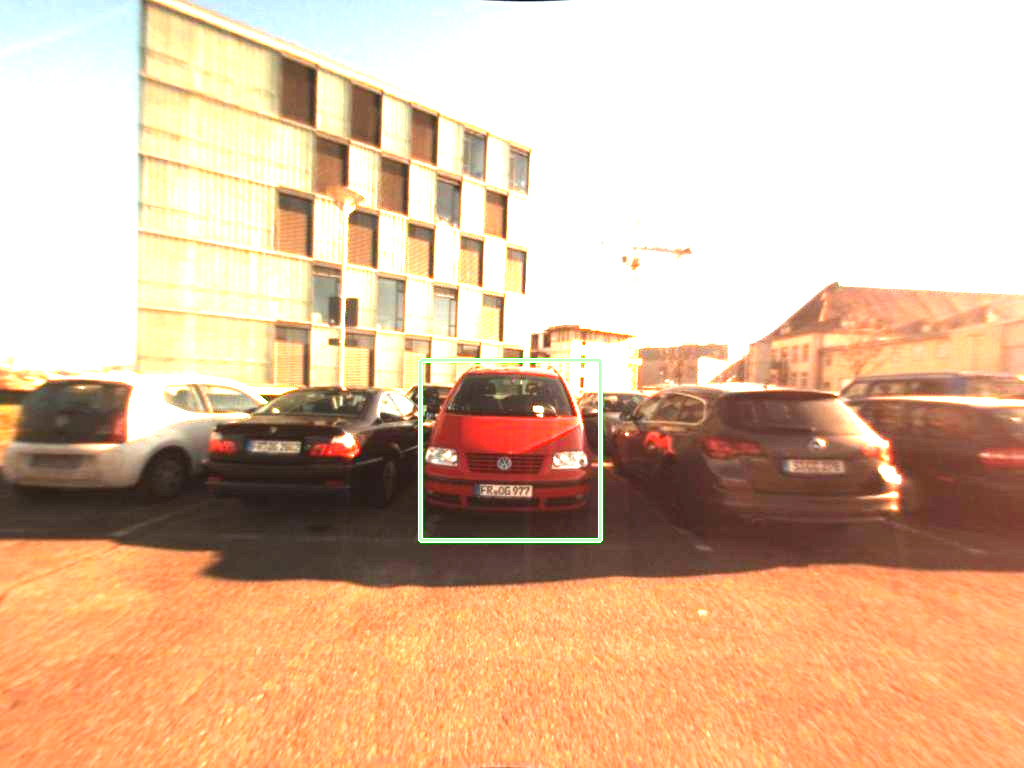
\includegraphics[width=0.31\textwidth]{pictures/det_7.jpg}}\hspace{2mm}
\subfloat{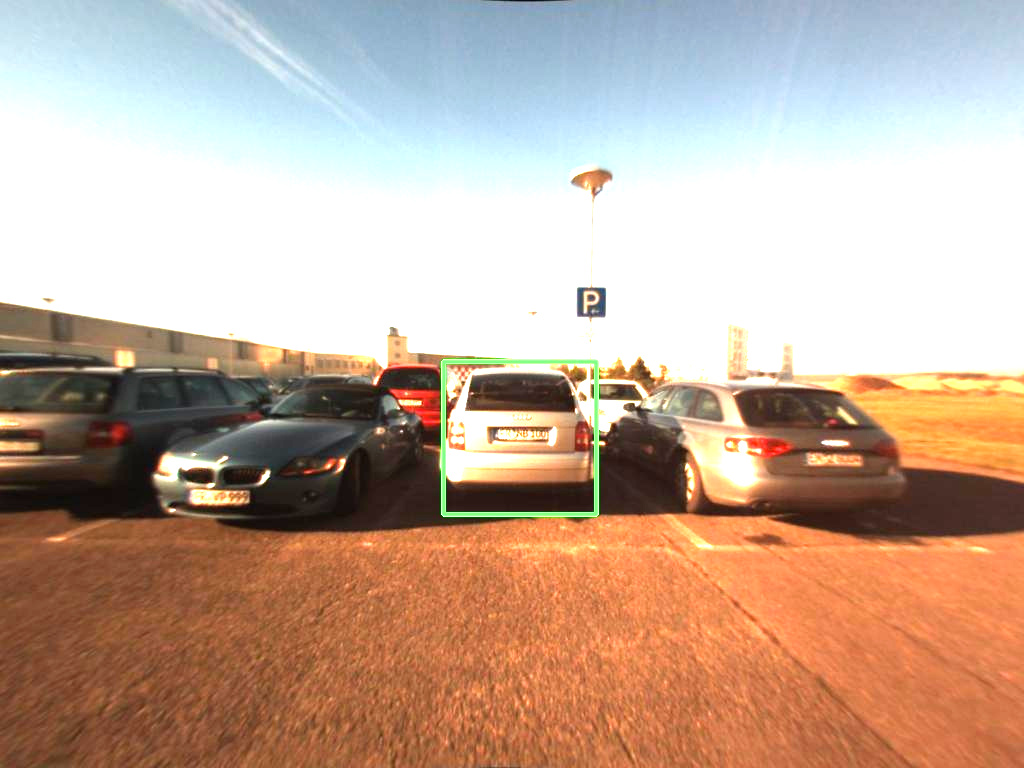
\includegraphics[width=0.31\textwidth]{pictures/det_8.jpg}}\hspace{2mm}
\subfloat{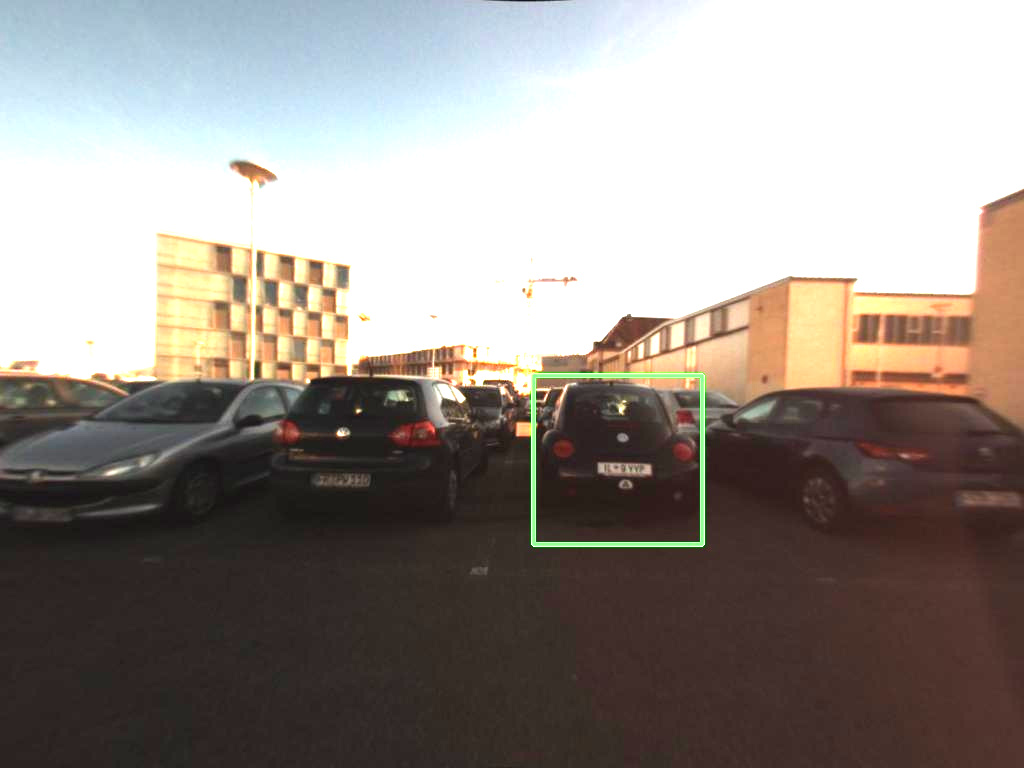
\includegraphics[width=0.31\textwidth]{pictures/det_9.jpg}}\\
\subfloat{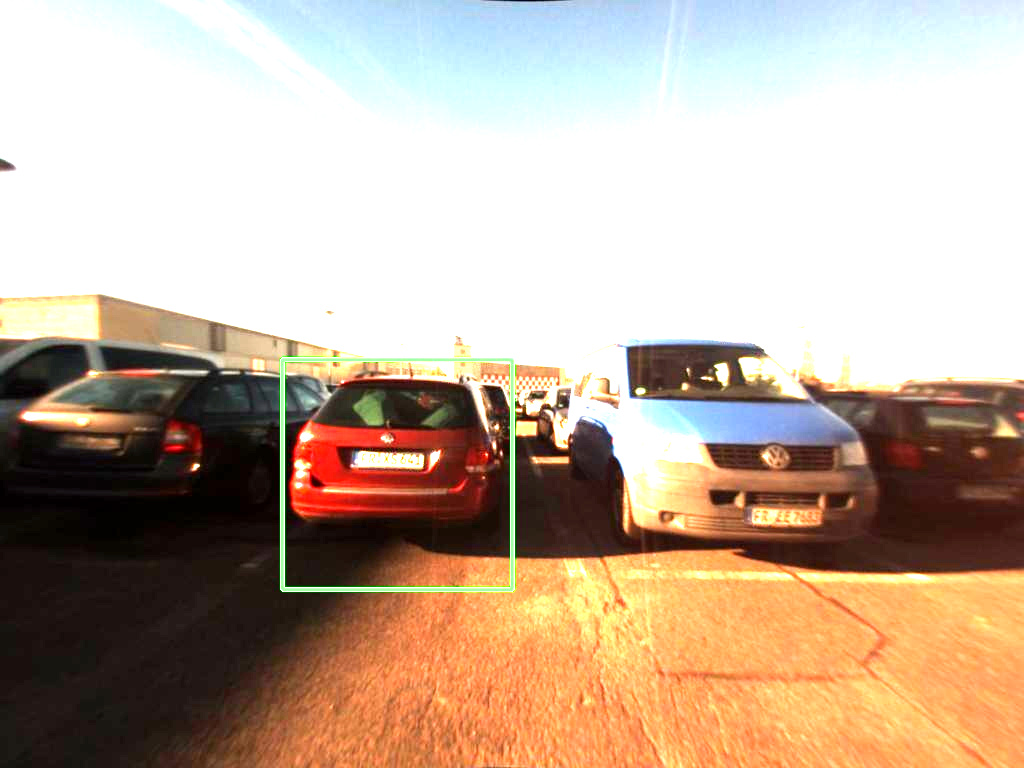
\includegraphics[width=0.31\textwidth]{pictures/det_10.jpg}}\hspace{2mm}
\subfloat{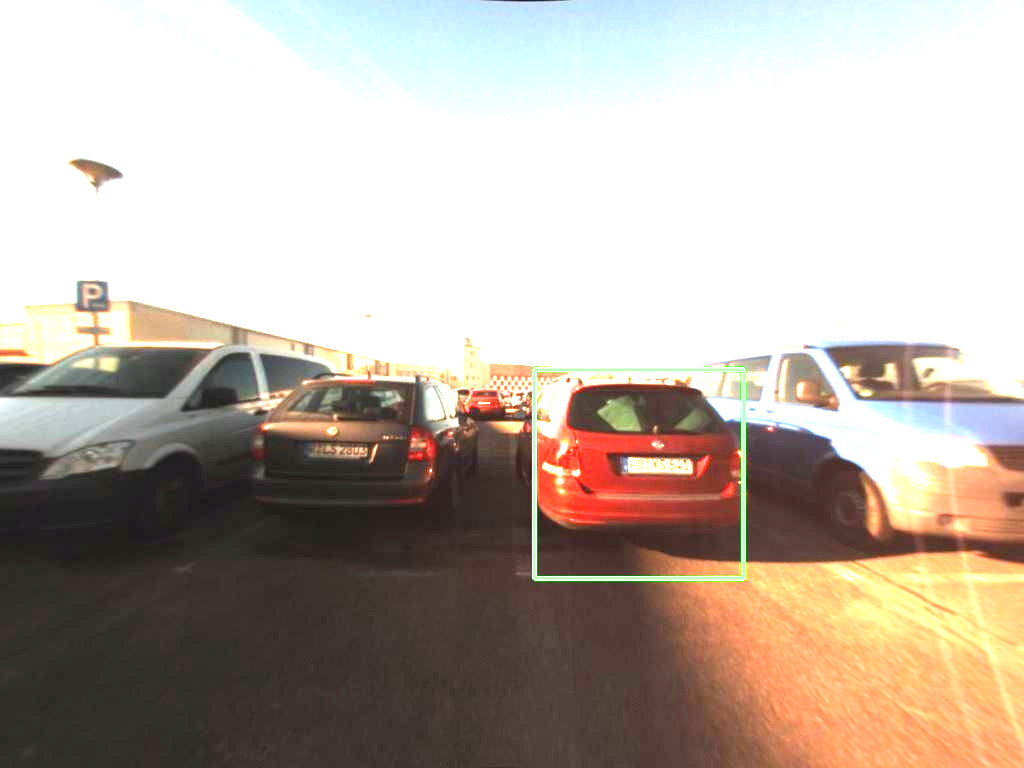
\includegraphics[width=0.31\textwidth]{pictures/det_11.jpg}}\hspace{2mm}
\subfloat{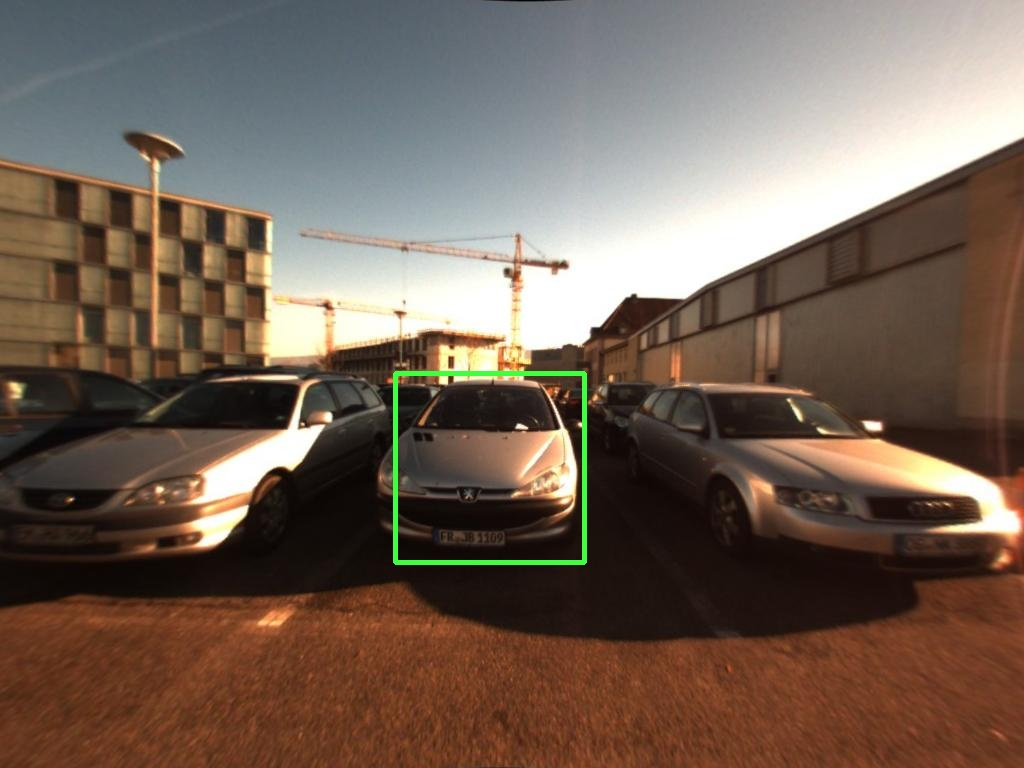
\includegraphics[width=0.31\textwidth]{pictures/det_12.jpg}}\\
\subfloat{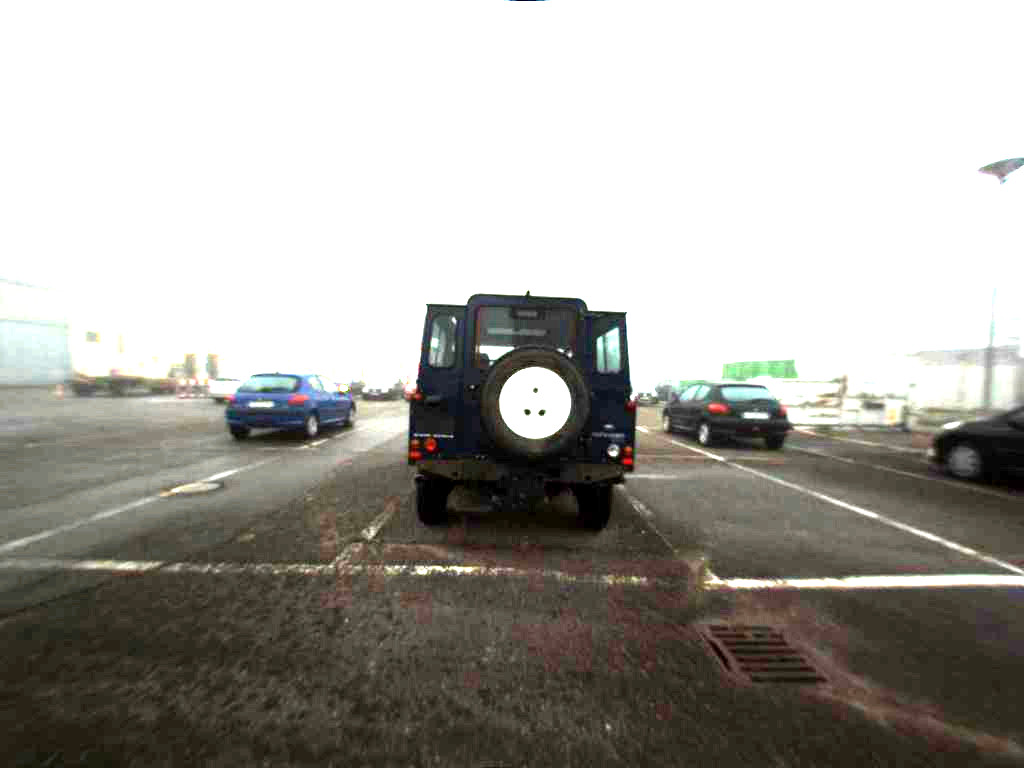
\includegraphics[width=0.31\textwidth]{pictures/undet_1.jpg}}\hspace{2mm}
\subfloat{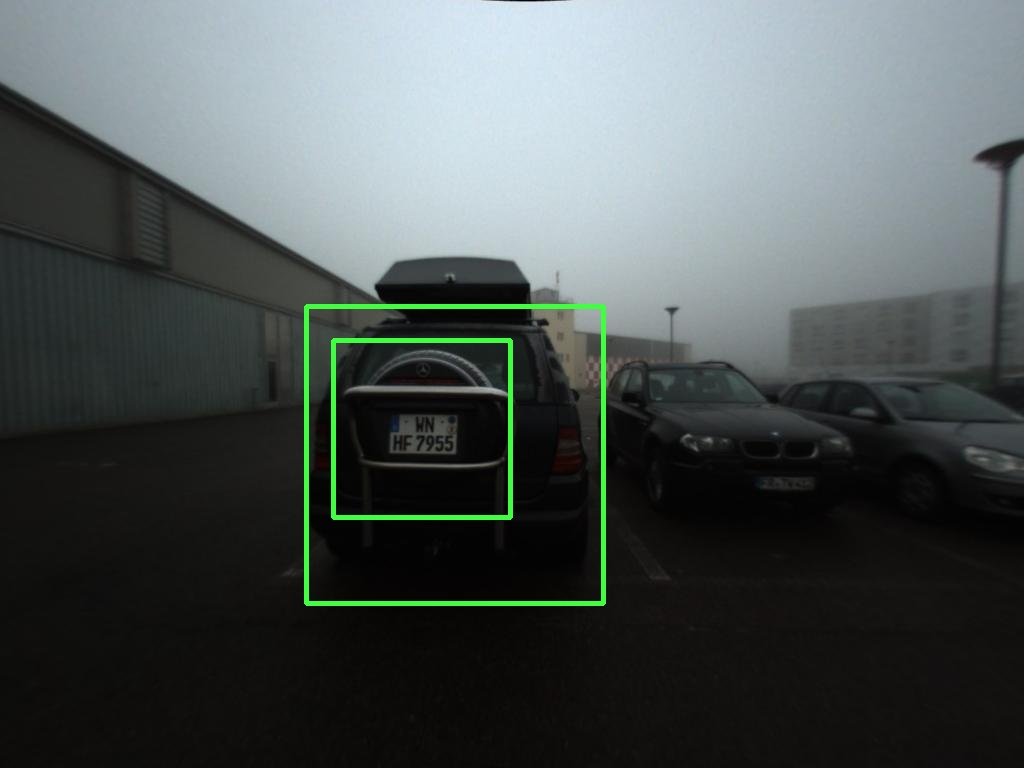
\includegraphics[width=0.31\textwidth]{pictures/undet_2.jpg}}\hspace{2mm}
\subfloat{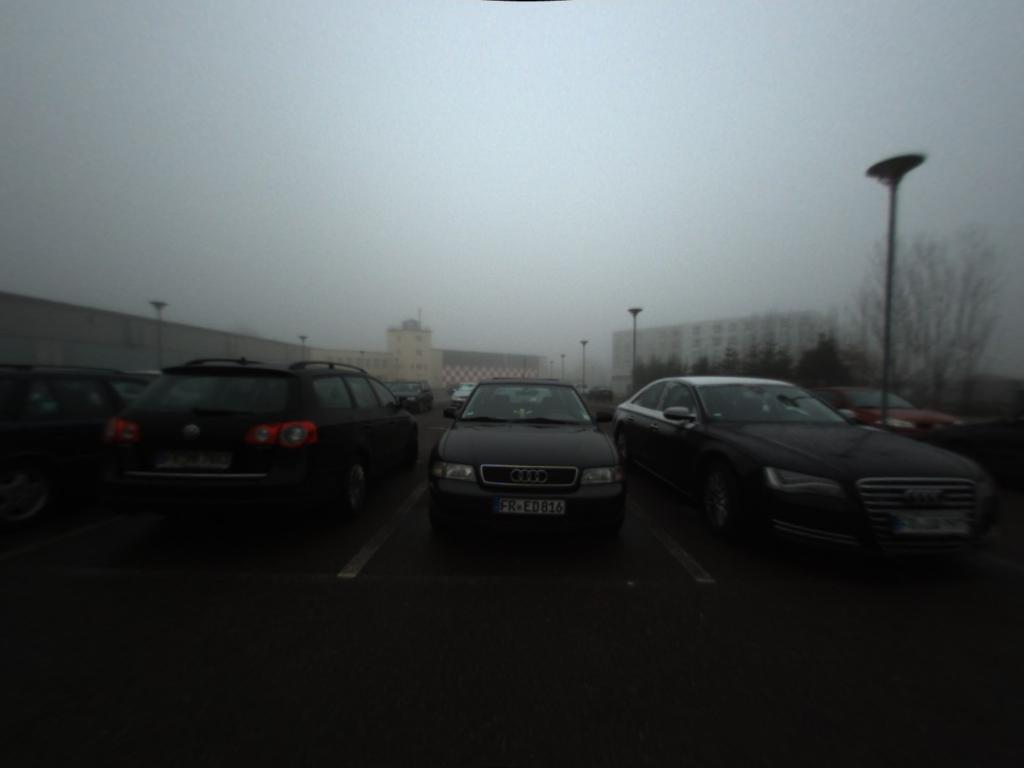
\includegraphics[width=0.31\textwidth]{pictures/undet_3.jpg}}\\
\caption{Examples of detections of different cars under different light conditions.}
\label{fig:detection_examples}
\end{figure}
